\section{An Application in Graph Drawing - Proof of \cref{one_bend_collinear_thm}}
\label{one_bend}
This section demonstrates an application of a connected dominating set in graph drawing. We establish that each planar graph with a small connected dominating set has a one-bend drawing with a large collinear set. We start with introducing a topological equivalent of one-bend collinear sets as in $\cite{DBLP:journals/jocg/LozzoDFMR18}$.


% We are interested in finding bounds on the size of $h$-bend collinear set. For $0$-bend collinear set, constructions of non-Hamiltonian cubic triconnected planar graphs \cite{DBLP:journals/jct/GrunbaumW73,DBLP:conf/wg/RavskyV11,DBLP:journals/jocg/LozzoDFMR18} imply that planar triangulation has a 0-bend collinear set of size at most $O(n^{\sigma})$ where $\sigma < 0.986$. Moreover, every planar triangulation has a 0-bend collinear set of size at least $\Omega(\sqrt{n})$ \cite{DBLP:journals/dcg/BoseDHLMW09} \cite{DBLP:journals/jgaa/Dujmovic17}. In a recent work, Dujmovic and Morin \cite{DBLP:conf/compgeom/DujmovicM19} show that every planar triangulation with maximum degree $\Delta$ has $0$-bend collinear set of size at least $\Omega(\frac{n^{0.8}}{\Delta^4})$.

% For the one-bend drawing of planar triangulation with $n$ vertices,  Everett et al. \cite{DBLP:conf/gd/EverettLLW07} show the existence of a set $\mathcal{U}$ of $n$ distinct points in the plane such that every $n$-vertex planar graph admits an embedding on vertex set $\mathcal{U}$ with at most one bend along each edge. Furthermore, Giacomo et al. \cite{DBLP:journals/comgeo/GiacomoDLW05} show that for a linear ordering $L$ of vertices of a planar triangulation $G$ and strictly convex curve $\lambda$, there is a one-bend planar drawing of $G$ such that vertices of $G$ appear on $\lambda$ with the same order in $L$.

% With further relaxation on the drawing of the edges, de Fraysseix et al. \cite{DBLP:journals/combinatorica/FraysseixPP90} show that any set of $n$ points in the plane is a universal set for the two-bend drawing of planar graphs. Furthermore, They show that the planar embedding problem of any $n$-vertex graph onto an $n$ collinear points in $\mathbb{R}^2$ with at most one bend along each edge is NP-complete.

\subsection{Characterisation of 1-Bend Collinear Sets}
A \defin{curve} $C$ is a continuous mapping from $[0, 1]$ to $\mathbb{R}^2$. We usually call $C(0)$ and $C(1)$ the \defin{endpoints} of $C$. If $C(0)=C(1)$ then  the curve is \defin{closed}. Otherwise, it is \defin{open}. A curve $C$ is called \defin{simple} if $C$ is $C(x) \neq C(y)$ for all $0\le x<y\le 1$ with the exception of $x=0$, $y=1$. $C$ is a \defin{Jordan Curve} if it is simple and closed.

Let $G$ be plane graph, a Jordan curve $C$ is a \defin{$k$-proper good curve} if it contains a point in the interior of some face of $G$ (\textit{good}), and the intersection between $C$ and each edge $e$ of $G$ is empty, or at most $k$ points, or the entire edge $e$ (\textit{proper}).

% Da Lozzo et al. 
\citet{DBLP:journals/jocg/LozzoDFMR18} characterize collinear sets in the straight line drawing of a planar graph using 1-proper good curves.

\begin{thm}[\cite{DBLP:journals/jocg/LozzoDFMR18} ] \label{straightline-topological}
Let $G$ be a plane graph. A set $S \subseteq V(G)$ is a collinear set if and only if there exists a $1$-proper good curve that contains $S$.
\end{thm}

The following lemma, illustrated in \cref{subdivisions}, gives a similar condition for one-bend collinear sets.

\begin{figure} [htbp]
  \centering
  \includegraphics[page=6]{figs/proper_good} \\
  $\Downarrow$ \\
  \includegraphics[page=7]{figs/proper_good}
  \caption{Subdividing $G$ so that a $2$-proper good curve $C$ becomes a $1$-proper good curve for the subdivided graph $G^+$.}
  \label{subdivisions}
\end{figure}

\begin{observation} \label{1-bend-topological}
    Let $G$ be a plane graph. A set $S \subseteq V(G)$ is a one-bend collinear set if $G$ has a $2$-proper good curve $C$ that contains $S$.
\end{observation}

\begin{proof}
Let $C$ be a 2-proper good curve that contains $S$. For each edge $e \in E(G)$ such that $|C \cap e| = 2$, we introduce a new subdivision vertex $u_e$ between the two intersection points of $C$ and $e$. By adding these new vertices, we obtain a plane drawing of a subdivision of $G$, denoted as $G^+$. Since every edge of $G^+$ is intersected by $C$ at most once, $C$ is $1$-proper good curve for $G^+$. Thus, by \cref{straightline-topological}, $S$ is a collinear set for $G^+$. Note that a straight line drawing of $G^+$ is a one-bend drawing for $G$. Therefore, $S$ is a one-bend collinear set for $G$.
\end{proof}


\subsection{From a Spanning Tree to a One-bend Collinear Set}

We prove that the leaves of a spanning tree of a planar graph induce a one-bend collinear set. Precisely, we prove the following theorem.

\begin{lem} \label{spanning_tree_to_collinear_set}
  Let $G$ be a planar graph and $T$ be a spanning tree of $G$. Then, the leaves of $T$ form a one-bend collinear set for $G$.
\end{lem}

\begin{proof}
    Let $\Gamma$ be a straight-line drawing of $G$.
    By \cref{1-bend-topological}, it is enough to introduce a 2-proper good curve $\ell$ on $\Gamma$ containing all the leaves of $T$. To navigate the curve $\ell$ on the drawing $\Gamma$, we construct an envelope around $\Gamma$ as follows. For each vertex $v \in V(G)$, we draw a small circle, $C_v$, centered at $v$. We make the radii of the circles small enough such that each vertex $v \in V(G)$, $C_v$ intersects only the edges incident to $v$ and it is disjoint from all the other circles that correspond to the other vertices. Moreover, for each edge $uv \in E(G)$, we draw two parallel segments on both sides of $uv$ with endpoints on the boundary of corresponding circles of $u$ and $v$. These parallel segments are close enough to the corresponding edges such that no two of them intersect. (see \cref{tree_walking}). Note that each edge $uv \in E(G)$ crosses the envelope exactly twice, once at $C_u$ and once at $C_v$.

    \begin{figure}
        \centering
        % \includegraphics[page=2]{figs/proper_good} \\
        % $\Downarrow$ \\
        \includegraphics[page=3]{figs/proper_good}\\
        $\Downarrow$ \\
        \includegraphics[page=4]{figs/proper_good}
        \caption{Constructing a $2$-proper good of $G$ that contains all the leaves of the tree $T$.}
        \label{tree_walking}
    \end{figure}


    Assume $T$ is rooted at an arbitrary vertex of degree at least 2. We build the curve $\ell$ on the envelope of $\Gamma$ as follows. Starting from the root, we traverse the tree in \textit{depth first search} order. For each edge $uv \in E(T)$, we add the segment on the right side of the traversal direction of $uv$ into the curve $\ell$.

    For each leaf $u$ of $T$, let $v_u$ be its neighbor in $T$. To include all the leaves of $T$ on the curve $\ell$, we join $u$ to the endpoint of segments around the edge $uv_u \in E(T)$ on $C_u$. To keep the curve $\ell$ closed, for each non-leaf vertex $u \in V(T)$, we append to $\ell$ the circular arcs from $C_u$ between the segments in $\ell$ in the order of the traversal. By the properties of the depth first traversal, $\ell$ is a closed curve. By construction, $\ell$ contains all the leaves of $T$ and all the other vertices of $T$ are inside $\ell$. Moreover, for each edge $uv \in E(G)$:

    \begin{enumerate}
        \item [(P1)] If $uv \in E(T)$ and neither $u$ nor $v$ is a leaf, then $|uv \cap \ell| = 0$,

        \item [(P2)] If $uv \in E(T)$ and either $u$ or $v$ is a leaf of $T$, then $|uv \cap \ell| = 1$, and

        \item [(P3)] If $uv \notin E(T)$, then $|uv \cap \ell| = 2$.
    \end{enumerate}

    Properties P1-P3 guarantee that $\ell$ is a 2-proper curve. Since the tree $T$ is not empty, $\ell$ intersects the circle of some vertex in $T$, so $\ell$ touches a face of $\Gamma$. Therefore, $\ell$ is $2$-proper good curve and by \cref{1-bend-topological}, there exists a one-bend collinear set for $G$ formed by the leaves of $T$.
\end{proof}

\begin{proof}[Proof of \cref{one_bend_collinear_thm}]
Let $G$ be an $n$-vertex planar graph. \cref{main_result2} implies that $G$ has a spanning tree with at least $11n/21$ leaves. Using this tree in \cref{spanning_tree_to_collinear_set} establishes \cref{one_bend_collinear_thm}.
\end{proof}
